\section{实数系的构造}

\summary{本节介绍了戴德金分割定义实数系，主要内容就是一步一步定义实数及实数系上的序和运算，验证其满足实数系的所有公理. }

\subsection*{Dedekind 分割法}

\textbf{I. 实数的定义}

\begin{definition}[Dedekind 分割]
设 $\alpha \subseteq \mathbb{Q}$ 满足：
\begin{enumerate}
    \item[(D1)] $\alpha \ne \varnothing$，且 $\alpha \ne \mathbb{Q}$；
    \item[(D2)] $\forall p,q \in \mathbb{Q}$，若 $q \in \alpha$ 且 $p<q$，则 $p \in \alpha$；
    \item[(D3)] $\alpha$ 无最大元. 
\end{enumerate}
则称 $\alpha$ 为一个 Dedekind 分割，即一个实数. 全体实数记为 $\mathbb{R}$. 
\end{definition}



记
\[
p^*:=\{q \in \mathbb{Q} \mid q<p\}.
\]

\textbf{II. 序关系}

定义
\[
\alpha \le \beta \iff \alpha \subseteq \beta.
\]

\begin{proof}[（O3）分离性的证明]
若 $\alpha \le \beta$ 不成立，则 $\alpha \not\subseteq \beta$，故存在 $p \in \alpha$ 使得 $p \notin \beta$. 

对任意 $q \in \beta$，若 $q>p$，则由 (D2) 有 $p \in \beta$，矛盾. 
故任意 $q \in \beta$ 都满足 $q<p$，从而 $q \in \alpha$. 

于是 $\beta \subseteq \alpha$，即 $\beta \le \alpha$. 
\end{proof}

\begin{theorem}[上确界存在定理]
$\mathbb{R}$ 中任何非空有上界集均有上确界. 
\end{theorem}

\begin{proof}
设 $E \subset \mathbb{R}$ 非空且有上界. 令
\[
\beta=\bigcup_{\alpha \in E}\alpha.
\]
又设 $\gamma$ 是 $E$ 的一个上界. 下证 $\beta \in \mathbb{R}$. 

$1^\circ$ （证 (D1)）

由 $E \ne \varnothing$，知 $\beta \ne \varnothing$. 

又因为 $\gamma \ne \mathbb{Q}$，可取 $p \in \mathbb{Q}$ 使 $p \notin \gamma$. 对任意 $\alpha \in E$，由 $\alpha \le \gamma$ 知 $\alpha \subseteq \gamma$，故 $p \notin \alpha$. 因此 $p \notin \beta$，于是 $\beta \ne \mathbb{Q}$. 

$2^\circ$ （证 (D2)）

若 $p \in \beta$ 且 $q<p$，则存在 $\alpha \in E$ 使 $p \in \alpha$. 由 $\alpha$ 满足 (D2)，得 $q \in \alpha$，于是 $q \in \beta$. 

$3^\circ$ （证 (D3)）

任取 $p \in \beta$，则存在 $\alpha \in E$ 使 $p \in \alpha$. 由于 $\alpha$ 中无最大元，存在 $q \in \alpha$ 使 $p<q$. 于是 $q \in \beta$，故 $\beta$ 中无最大元. 

因此 $\beta$ 是一个分割，即 $\beta \in \mathbb{R}$. 

对任意 $\alpha \in E$，有 $\alpha \subseteq \beta$，故 $\alpha \le \beta$，所以 $\beta$ 是 $E$ 的一个上界. 

若 $\sigma$ 也是 $E$ 的一个上界，则对任意 $\alpha \in E$，都有 $\alpha \le \sigma$，即 $\alpha \subseteq \sigma$. 于是
\[
\beta=\bigcup_{\alpha \in E}\alpha \subseteq \sigma,
\]
故 $\beta \le \sigma$. 因此 $\beta=\sup E$. 
\end{proof}

\begin{notebox}
原图末行写作
\[
\alpha=\sup\{p^* \mid p<\alpha\}=\sup\{p^* \mid p\le \alpha\}.
\]
其中集合条件处字迹略糊；第二个条件也可能是 $p^* \le \alpha$，这里只按可辨笔迹照录并标注. 
\end{notebox}

\textbf{III. 加法}

定义
\[
\alpha+\beta=\sup E_{\alpha,\beta},
\]
其中
\[
E_{\alpha,\beta}:=\{(p+q)^* \mid p^* \le \alpha,\ q^* \le \beta\}.
\]

\begin{proposition}
若 $\forall s>0$，都有 $\alpha \le \beta+s^*$，则 $\alpha \le \beta$. 
\end{proposition}

\begin{proof}
假设 $\alpha>\beta$，则可取 $p,q \in \mathbb{Q}$ 使
\[
\alpha>p^*>q^*>\beta.
\]
于是
\[
\beta+(p-q)^*<q^*+(p-q)^*=p^*<\alpha,
\]
与题设矛盾，故 $\alpha \le \beta$. 
\end{proof}

\textbf{IV. 乘法}

当 $\alpha>0^*$，$\beta>0^*$ 时，定义
\[
\alpha\beta:=\sup M_{\alpha\beta},
\]
其中
\[
M_{\alpha\beta}:=\{(pq)^* \mid 0<p^* \le \alpha,\ 0<q^* \le \beta\}.
\]

并约定
\[
\alpha\beta=
\begin{cases}
0^*, & \alpha=0^* \text{ 或 } \beta=0^*,\\
-((-\alpha)\beta), & \alpha<0^*,\ \beta>0^*,\\
-(\alpha(-\beta)), & \alpha>0^*,\ \beta<0^*,\\
(-\alpha)(-\beta), & \alpha<0^*,\ \beta<0^*.
\end{cases}
\]

\textbf{V. 完备性}

\newpage
% 本页四边边距全部设为0
\newgeometry{left=0pt,right=0pt,top=0pt,bottom=0pt}
% 去掉页眉页脚
\thispagestyle{empty}
\noindent% 取消首行缩进
% 插入图片，宽高等于整张纸张大小
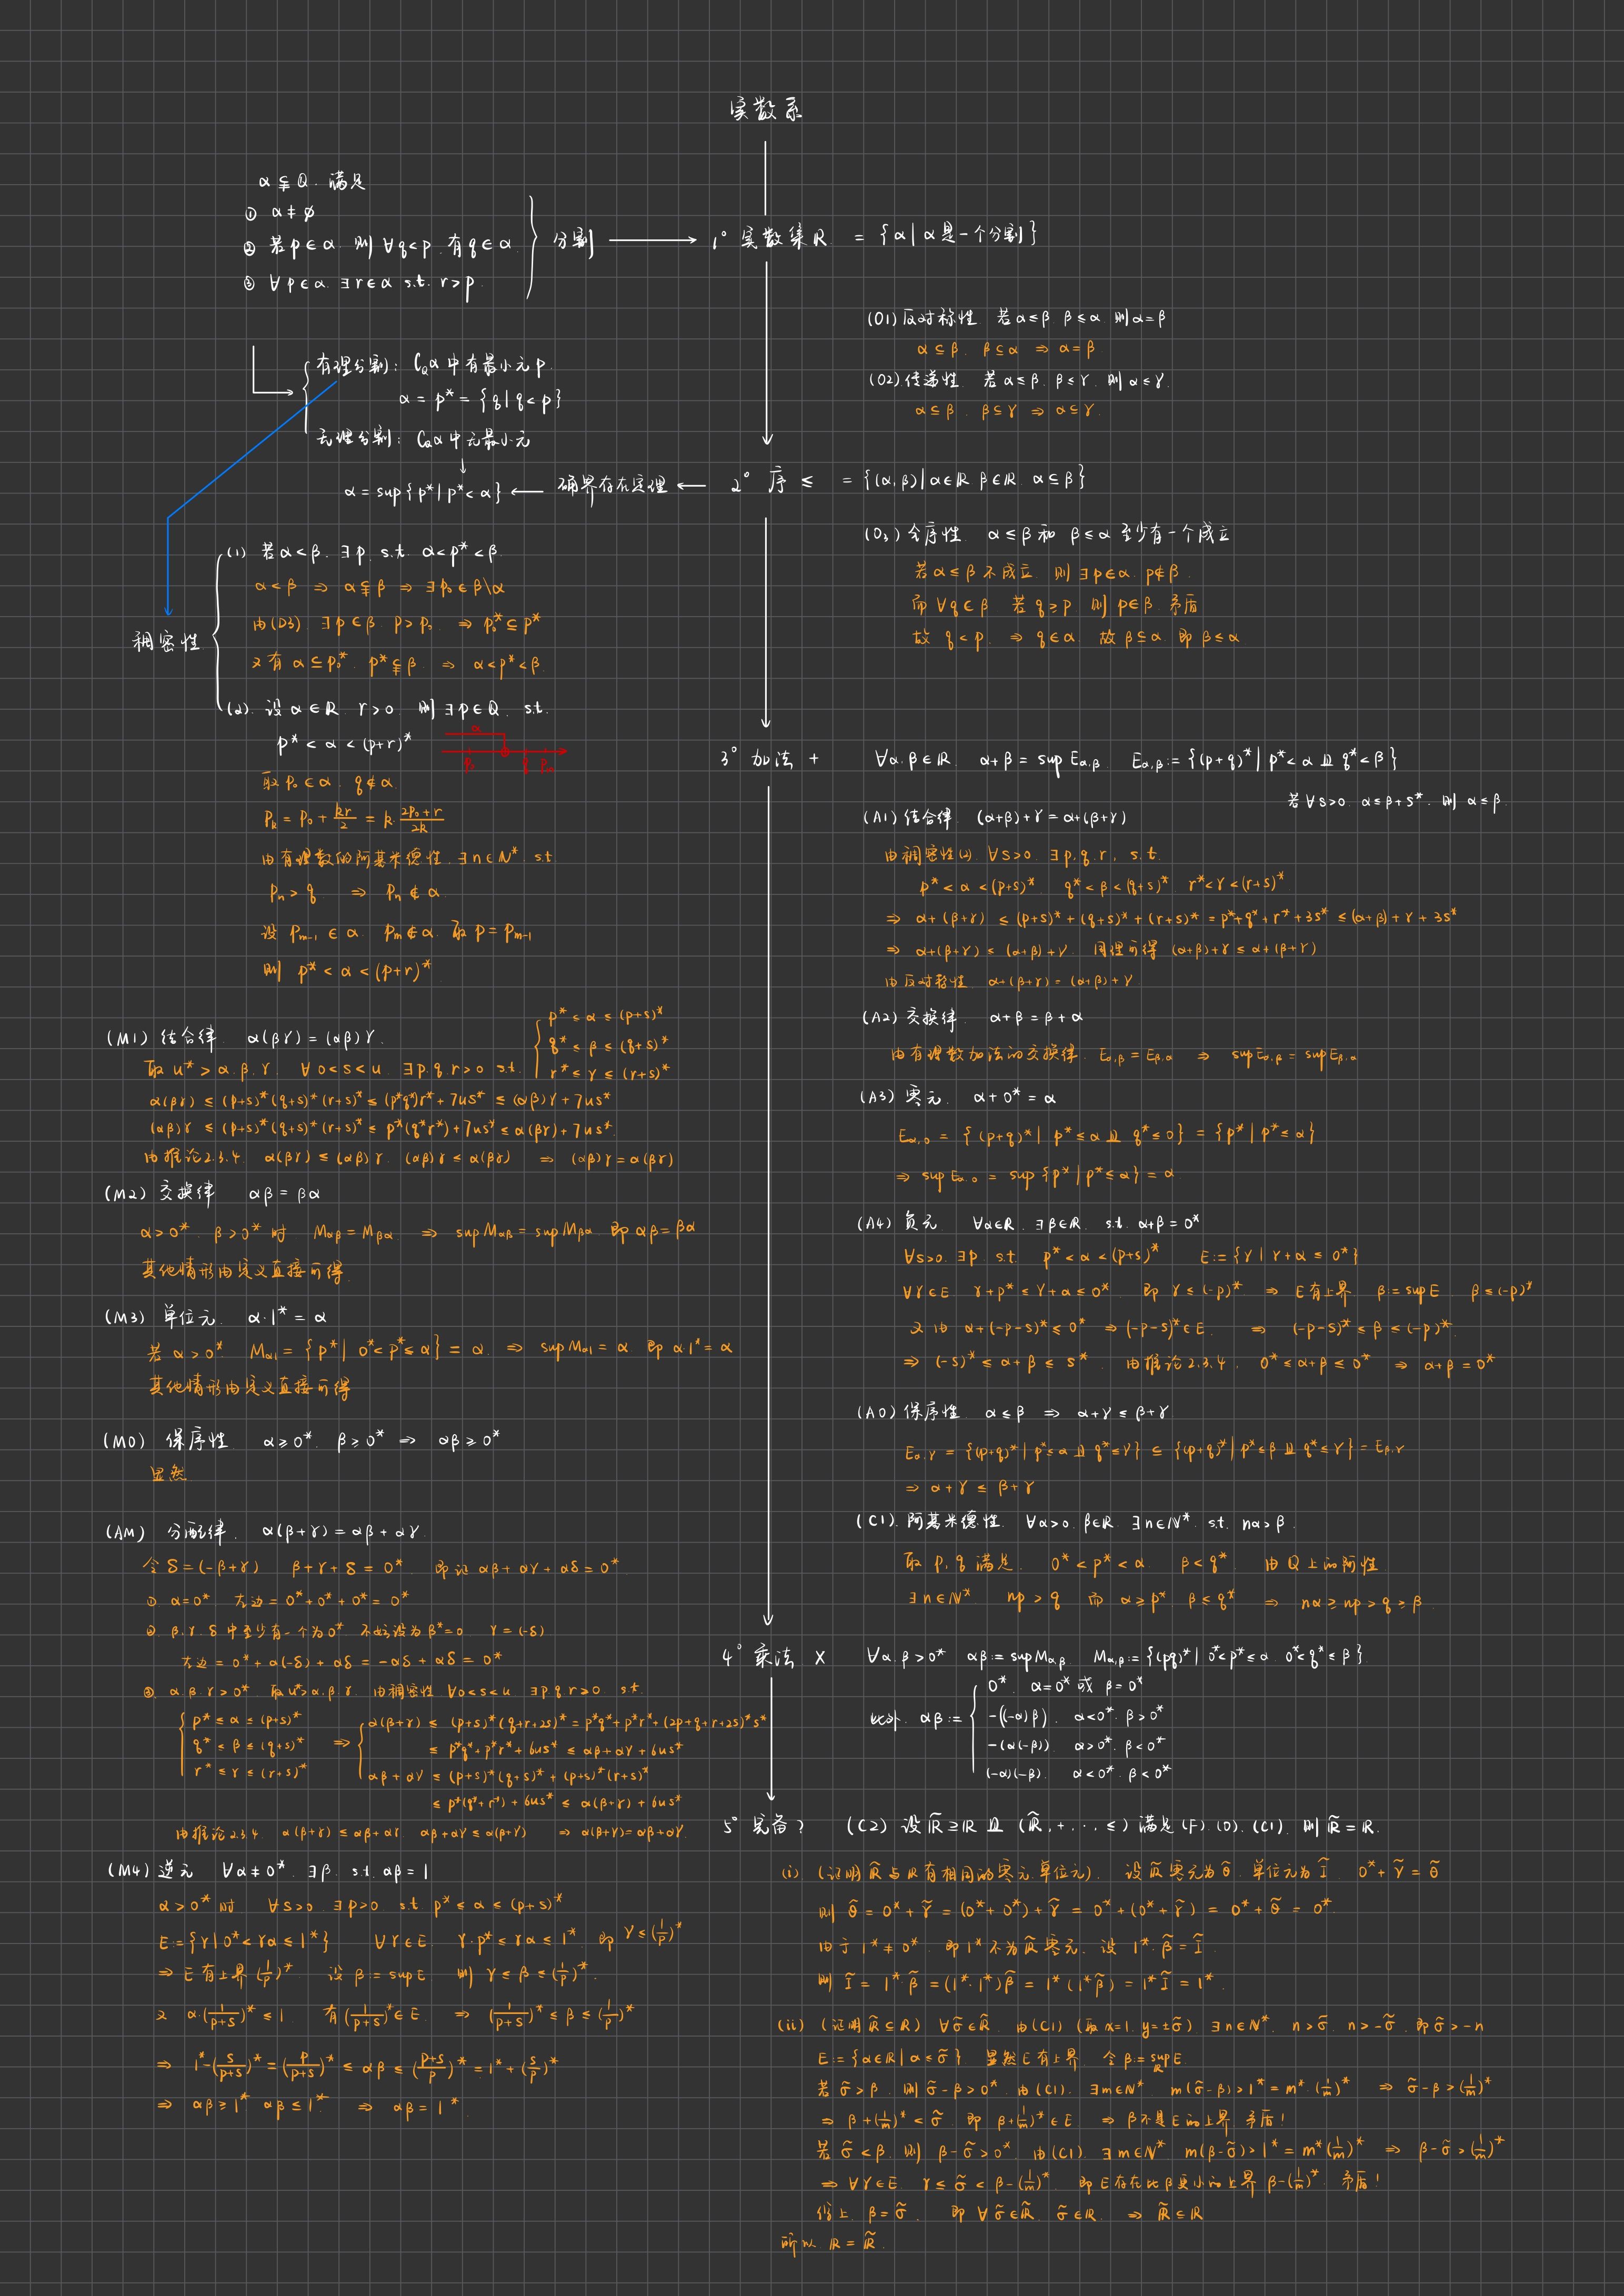
\includegraphics[width=\paperwidth,height=\paperheight]{数学分析/ch2-实数系/实数系.jpg}
% 恢复文档原来的页边距
\restoregeometry